\documentclass{article}[18pt]
\usepackage{../../../../format}
\lhead{Networks and Systems - Security}


\begin{document}
\begin{center}
\underline{\huge Operating System Security \& Access Control}
\end{center}
\section{Access Control}
\begin{itemize}
	\item Your computer contains lots of subjects (typically users, people) and lots of objects (typically documents, images, programs
	\item Who chooses access rights?
	\begin{itemize}
		\item The file owner - Mandatory Access Control (MAC)
		\item The system owner - Discretionary Access Control (DAC)
		\item Anyone who has rights
	\end{itemize}
	\item What/how/where do we store access permissions? Multiple approaches
\end{itemize}
\section{Access Control Matrix (ACM)}
\begin{itemize}
	\item [+] Easy to define, easy to verify
	\item [-] Poor scalability, poor handling of changes, could get corrupted
\end{itemize}
\begin{center}
	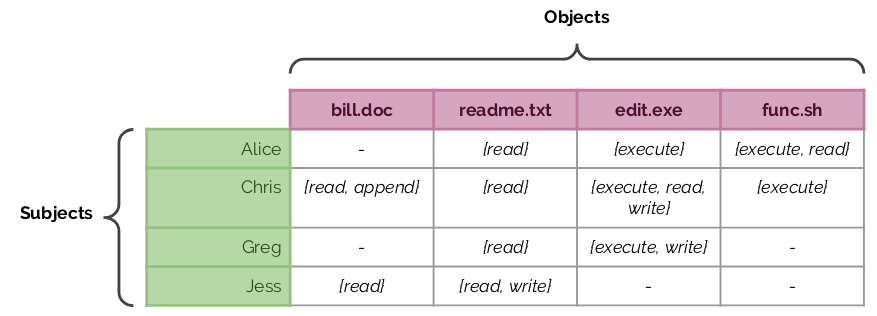
\includegraphics[scale=0.7]{ACM}
\end{center}
Dashes represent no access rights\\
Append typically used for log files
\section{Access Permissions}
*NIX has 8 access permission settings for 3 types of users
\begin{itemize}
	\item Owners, Groups and Others
	\item Combination of read(r), write(w), and execute (x)
	\item Represented as numbers in base 8
\end{itemize}
\begin{center}
	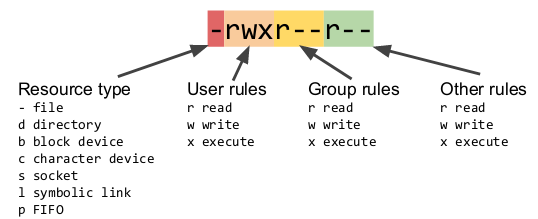
\includegraphics[scale=0.7]{permission}
\end{center}
\texttt{chown} and \texttt{chmod} can be used to modify access permissions
\section{setuid, setgid, and sticky bits}
\textbf{setuid bit}: Users run executable with permissions of the executable owner\\
\textbf{sticky bit}: Prevents users with write/execute permissions from deleting the directory contained files (typically on \texttt{tmp} folder)
\section{*NIX Permissions to ACM}
\begin{center}
	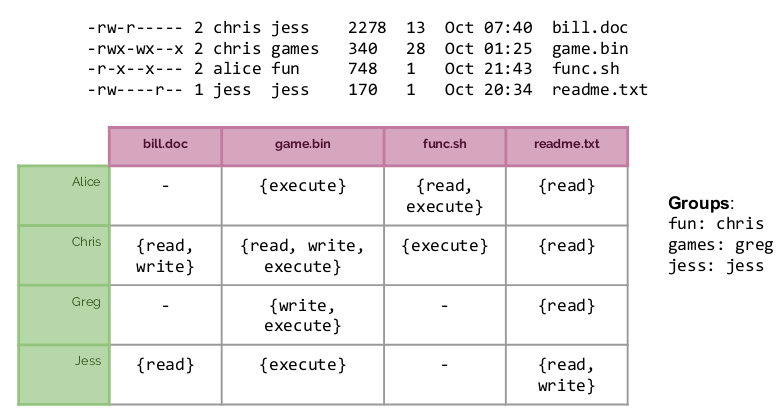
\includegraphics[scale=0.7]{permission1}
\end{center}
\section{Link Vulnerabilities}
\begin{itemize}
	\item Add new path to an inode
	\item Multiple names for a single inode
	\item For example, to overwrite /etc/password
	\begin{lstlisting}
	ln -s /etc/passwd file
	trusted_dump file < *passwd-entry*
	\end{lstlisting}
	e.g. a command which can read/write root owned files, but doesn't know the file is /etc/passwd
	\item Programs have to be aware of which files they are using
	\item \texttt{0\_NOFOLLOW} flag can be added to prevent following links e,g. \texttt{open(file, 0\_NOFOLLOW, mode)}
\end{itemize}
\section{Hardening (Not examined)}
\begin{itemize}
	\item SELinux - Make sure that programs only access what they're meant to
	\item AppArmor - Similar but simpler than SE linux
\end{itemize}
\section{Device File Vulnerabilities}
Devices are represented as files
\begin{itemize}
	\item \texttt{/dev/tty} - terminal
	\item \texttt{/dev/mem} - physical memory
	\item \texttt{/dev/kmem} - virtual memory
	\item \texttt{/dev/mouse} - mouse
\end{itemize}
Created using mknod (only accessible by root)
\begin{itemize}
	\item Can bypass access control by getting access to memory
	\item Can get access to user inputs
\end{itemize}
\section{Access Control Lists}
\begin{itemize}
	\item Store by column (object focused)
	\item [+] Easy to view object access control, easy to remove access rights if object removed
	\item [-] Poor overview of access rights per subject, difficult to remove subject
\end{itemize}
\begin{center}
	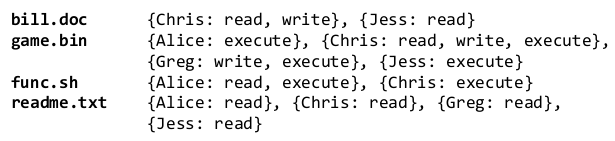
\includegraphics[scale=0.7]{ACL}
\end{center}
\section{Capability-based Security}
\begin{itemize}
	\item Store by row (subject-focused)
	\item [+] Easy to transfer ownership, easy inheritance of access rights
	\item [-] Poor overview of access rights per object, difficulty of revocation of object
\end{itemize}
\begin{center}
	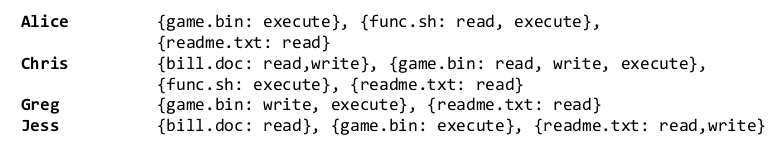
\includegraphics[scale=0.7]{capability}
\end{center}
\section{Windows}
\begin{itemize}
	\item Windows registry
	\begin{itemize}
		\item Core place for system control
		\item Target for hackers
		\item Controls multiple computers
	\end{itemize}
	\item Windows domain
	\begin{itemize}
		\item Computers sharing things such as passwords
	\end{itemize}
	\item Principles
	\begin{itemize}
		\item SAM format - old but used in most places
		\item UPN - more modern
	\end{itemize}
	\item Login - Happens in different ways depending if the computer is alone or part of a network
	\item More levels than *NIX
	\begin{itemize}
		\item Hardware, System, Administrator, Users
	\end{itemize}
	\item Library loading is a problem
	\item Viruses are very common and easy
	\item Windows adding features to make OS less predictable
	\begin{itemize}
		\item Image randomization (OS boots in one of 256 configurations)
		\item Services restart if failed (not the best practise for security)
		\begin{itemize}
			\item Vista+ sets some critical services to only restart twice, then manual restart
		\end{itemize}
	\end{itemize}
	\item NTFS is much more secure than FAT32 \& DOS
	\begin{itemize}
		\item Adds two ACLs:
		\begin{itemize}
			\item DACL: Reading, writing, executing, deleting by which users or groups
			\item SACL: for defining which actions are audited/logged, e.g.on activity being successful/failed
		\end{itemize}
		\item Compression, encryption
	\end{itemize}
\end{itemize}
\section{Bell-LaPadula Model}
Bell-LaPadula confidentiality policy, "read down, write up"
\begin{itemize}
	\item Simple security property
	\begin{itemize}
		\item Subject (Greg) cannot read object of higher sensitivity
	\end{itemize}
	\item Star property (* property)
	\begin{itemize}
		\item Subject cannot write to object of lower sensitivity. This is because Greg might know things that shouldn't be able to be accessed by people of lower security
	\end{itemize}
	\item Strong star property (Strong * Property)
\end{itemize}
\begin{center}
	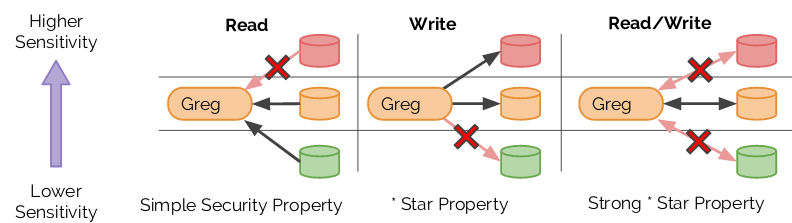
\includegraphics[scale=0.7]{Bell-LaPadula}
\end{center}
\section{Biba integrity model}
Biba integrity model - "read up, write down"
\begin{itemize}
	\item Simple Security property
	\begin{itemize}
		\item Subject (Greg) cannot read object of lower integrity (can only read data that is as good or better than his)
	\end{itemize}
	\item Star property (* property)
	\begin{itemize}
		\item Subject cannot write to object of higher integrity (can only write data that is as good or worse than his)
	\end{itemize}
	\item Invocation property
	\begin{itemize}
		\item Subject/process cannot request higher integrity access
	\end{itemize}
\end{itemize}
\begin{center}
	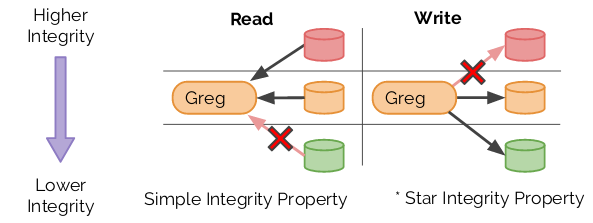
\includegraphics[scale=0.7]{biba}
\end{center}
\section{Clark-Wilson Integrity Model}
\begin{itemize}
	\item Bell-LaPadula is good for confidential systems
	\item Biba is good for integrity-preserving systems
	\item What about businesses/industry processes where you need both? Clark-Wilson Model
	\begin{itemize}
		\item Limits direct interaction between subjects and objects
		\item Prevent unauthorized subjects from modifying objects
		\item Prevent authorized subjects from making invalid modifications to objects
		\item Maintain internal/external consistency
	\end{itemize}
\end{itemize}
\begin{center}
	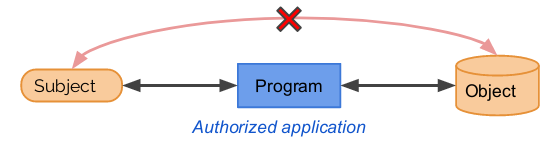
\includegraphics[scale=0.7]{Clark-Wilson}
\end{center}
\section{Protection Rings}
\begin{itemize}
	\item Hardware based access control - also used to protect data and functionality from faults
	\item Each subject and object are assigned a number based on importance
	\item Decisions are made by comparing numbers (if subject $<$ object, disallow access)
	\item x86 CPUs offer four rings, but typically (Windows/UNIX) only two (0,3) are used
	\item ARM implements 3 levels (application, operating system and hypervisor)
\end{itemize}
\begin{center}
	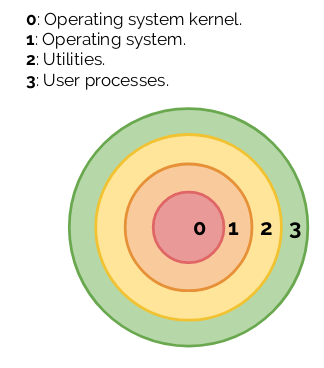
\includegraphics[scale=0.7]{protection_ring}
\end{center}

\section{Securing BIOS and Bootloader}
BIOS should have a password for changing the settings
\begin{itemize}
	\item If you have physical access, then you can reset BIOS easily by resetting the CMOS
	\item So lock the machine physically (require a key)
\end{itemize}
Bootloader (e.g. GRUB) should have a password for changing the settings

\end{document}